\documentclass{article}
\usepackage{amsmath}
\usepackage{amsfonts}
\usepackage{amssymb}
\usepackage{tikz}
\usetikzlibrary{arrows}
\usetikzlibrary{decorations.markings}

\begin{document}

\textit{A2 Physics OCR 2016 Exam}\\
\section*{Ultrasound}

Ultrasound waves are similar to sound waves, i.e. longitudinal waves, but of frequency $>$ 20 kHz, so inaudible to humans. In medical applications waves of the order of MHz are used which usually travel through tissue, rather than air.


\subsection*{The Piezoelectric Effect}

Certain crystals contract when a pd is applied to them. This can be used to produce ultrasound of frequencies of the order of MHz.
This process also works in reverse: changes of pressure produce a corresponding variable p.d. So the same crystal can be used as a receiver.


\subsection*{The Principle of Ultrasound Scanning}

When ultrasound travels from one medium, e.g. flesh, to another, e.g. bone, where its speed is different, part of the wave energy is reflected. This echo can be picked up and fed into a computer to obtain information. (Information being a measurement or an image, see A- and B-Scan below.)

\begin{itemize}
\item{A short burst of ultrasound is produced by a transducer and sent into the body.}
\item{There is a pause while reflected echoes come back to be picked up by the same transducer.}
\item{This means there is a maximum pulse repetition frequency (of about 1 kHz).}
\end{itemize}
\scriptsize{\textit{[Get them to look at and understand graphs on page 201]}}\\
\normalsize

\subsection*{Type A Scans (aka A-Scans) and Type B Scans (aka B-Scans)}

Type A, or Amplitude-scans, allow measurements to be taken to determine dimensions of objects inside the body, e.g. the size of a foetus. No image is produced.\\

Type B, or Brightness-scans, allow an image to be formed. The amplitude of the reflected pulses are displayed as the brightness of a spot on the screen that sweeps vertically down. An array of transducers are used to produce a two dimensional image.


\subsection*{Acoustic Impedance Z}

Is defined as
\begin{displaymath}
Z = \rho c
\end{displaymath}
where $\rho=\text{density of the material}$ and $c=\text{the speed of ultrasound in the material}$.

\subsection*{Acoustic Impedence}
When ultrasound hits a boundary
\begin{itemize}
\item{part of its intensity is \textbf{reflected} and}
\item{part of its intensity is \textbf{transmitted} (refracted)}
\end{itemize}
\begin{figure}[h]
\centering
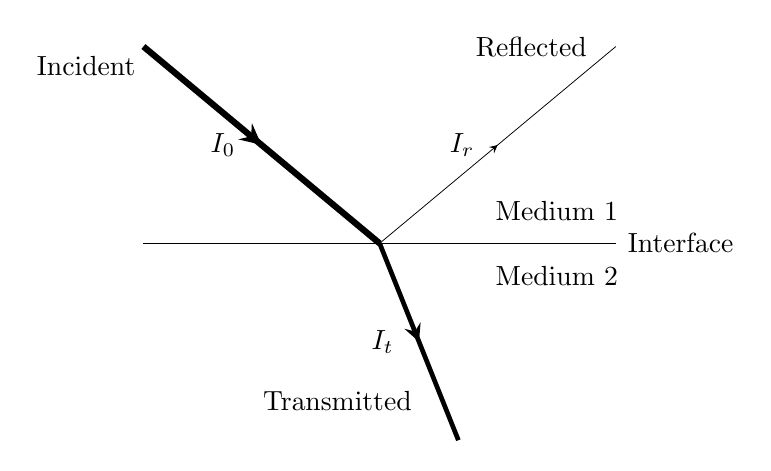
\begin{tikzpicture}
%\draw[help lines] (0,0) grid (6,5);

\draw[ultra thin](0,2.5)--(6,2.5) node[very near end,above=5pt] {Medium 1} node[very near end,below=5pt] {Medium 2} node[at end,right=1pt] {Interface};
\draw[
	line width=.8mm,
	decoration={
		markings,
		mark=at position .5 with{\arrow{stealth};}},
	postaction={decorate}](0,5)--(3,2.5) node[pos=.1, left=7pt] {Incident}node[pos=.5, left=5pt] {$I_0$};
\draw[line width=.6mm,
	decoration={
		markings,
		mark=at position .5 with{\arrow{stealth};}},
	postaction={decorate}](3,2.5)--(4,0) node[pos=.8, left=7pt] {Transmitted}node[pos=.5, left=5pt] {$I_t$};
\draw[line width=.1mm,
	decoration={
		markings,
		mark=at position .5 with{\arrow{stealth};}},
	postaction={decorate}](3,2.5)--(6,5) node[pos=1, left=7pt] {Reflected}node[pos=.5, left=5pt] {$I_r$};



\end{tikzpicture}
\label{Figure:IncidentTransmittedReflected}
\caption{The incident ray $I_0$ strikes the interface between Medium 1 and Medium 2. Part of the incident intensity is transmitted (refracted) into Medium 2 and part of it is reflected back into Medium 1.}
\end{figure}
\noindent
We have
\begin{displaymath}
\frac{I_r}{I_0}=\left(\frac{Z_2-Z_1}{Z_2+Z_1}\right)^2
\end{displaymath}
where $Z_i$ is the acoustic impedance for medium $i$ and $I_r$ and $I_0$ are the reflected and the incident intensities respectively.

\end{document}